\documentclass[a4paper,14pt]{extarticle}

\usepackage[T2A,T1]{fontenc}
\usepackage[utf8]{inputenc}
\usepackage[english,russian]{babel}
\usepackage{csquotes}

% PDF search & cut'n'paste
\usepackage{cmap}

%% Поля
\usepackage[includeheadfoot,top=20mm,bottom=20mm,left=30mm,right=15mm]{geometry}

%% Отступ в первом абзаце
\usepackage{indentfirst}

%% Включение графических файлов.
\usepackage{graphicx}

%% Appendix.
\usepackage[titletoc,title]{appendix}
\renewcommand{\appendixtocname}{Приложения}
\renewcommand{\appendixpagename}{Приложения}
\renewcommand{\appendixname}{Приложние}
\makeatletter
\let\oriAlph\Alph
\let\orialph\alph
\renewcommand{\@resets@pp}{\par
  \@ppsavesec
  \stepcounter{@pps}
  \setcounter{section}{0}%
  \if@chapter@pp
    \setcounter{chapter}{0}%
    \renewcommand\@chapapp{\appendixname}%
    \renewcommand\thechapter{\@Alph\c@chapter}%
  \else
    \setcounter{subsection}{0}%
    \renewcommand\thesection{\@Alph\c@section}%
  \fi
  \if@pphyper
    \if@chapter@pp
      \renewcommand{\theHchapter}{\theH@pps.\oriAlph{chapter}}%
    \else
      \renewcommand{\theHsection}{\theH@pps.\oriAlph{section}}%
    \fi
    \def\Hy@chapapp{appendix}%
  \fi
  \restoreapp
}
\makeatother

%% Рисунки в приложении содержат номер приложения: 'A.1'.
\usepackage{chngcntr}

%% Russian-styled figure and table captions.
\usepackage[labelsep=period,font=it]{caption}

% Here we define the relationships for the counters: normaly we should
% reset the figure & table counters every chapter.
\makeatletter
\@addtoreset{figure}{section} % Figure counter
\@addtoreset{table}{section} % Table counter
\makeatother

%% Include paragraphis into TOC.
\setcounter{secnumdepth}{5}
\setcounter{tocdepth}{5}

%% Newline after paragrpaph title.
\makeatletter
\renewcommand\paragraph{%
   \@startsection{paragraph}{4}{0mm}%
      {-\baselineskip}%
      {.1\baselineskip}%
      {\normalfont\normalsize\bfseries}}
\makeatother

%% Drop chapter number and
% \usepackage{titlesec}
% \renewcommand{\thesection}{\arabic{section}}
% \renewcommand{\thesubsection}{\arabic{subsection}}

\usepackage[titles]{tocloft}

%% Inline-списки.
\usepackage[inline]{enumitem}
\AddEnumerateCounter{\asbuk}{\@asbuk}{\cyrm}

\makeatother
\renewcommand{\labelitemi}{--}

% Keeps floats `in their place', preventing them from floating past a
% "\FloatBarrier" command into another section.  The floats should not move
% past every "\section".
\usepackage[section]{placeins}

\usepackage[%
    backend     = biber,
    bibencoding = utf8,
    hyperref    = false,
    citestyle   = gost-footnote-min,
    bibstyle    = gost-footnote
]{biblatex}
\addbibresource{references/chapter2.bib}

%% Ссылочки.
\usepackage{hyperref}
\makeatletter
\let\abx@macro@autociteOrig\abx@macro@autocite
\renewbibmacro{autocite}{%
   \bibhyperref{%
   \let\bibhyperref\relax\relax%
   \abx@macro@autociteOrig%
   }%
}%
\makeatother

%% Separate multiple cites with '; '
\renewcommand\multicitedelim{\addsemicolon\space}

\usepackage{remreset}
\makeatletter\@removefromreset{footnote}{chapter}\makeatother

%% Полуторный интервал
\usepackage[nodisplayskipstretch]{setspace}

%% Переименование "содержания" в "оглавление"
\gappto\captionsrussian{\renewcommand{\contentsname}{Оглавление}}

\addtolength{\textheight}{\headheight}
\addtolength{\textheight}{\headsep}
\setlength{\headsep}{0pt}
\setlength{\headheight}{0pt}

%% Преобразует footnote '2 3' -> '2, 3'.
\usepackage[multiple]{footmisc}

\begin{document}

% ------------------------------------------------------------------------------
% Оглавление
\thispagestyle{empty} % Disabling numbering on the TOC page.
\tableofcontents

% ------------------------------------------------------------------------------
% Текст работы
\begin{onehalfspacing}
  \section{Тенденции в современном лого-дизайне и эмблематическая сущность логотипа}

\subsection{Современные тенденции в лого-дизайне и проблемы классификации}

В заключение первой главы мы сделали вывод о том, что экспонента, смысловое содержание логотипа
находятся в прямой зависимости от конкурентоспособности компании-производителя  и производимых ею
товаров и услуг.  Конкурентная борьба стимулирует производителя постоянно искать и находить новые
пути эффективного сбыта продукции. Массовое производство, массовое потребление и массовая культура
естественным образом предполагают массовое производство, распространение и закрепление в массовом
сознании знаков мгновенной идентификации -- логотипов. По этой причине именно оригинальный, необычный
лого-дизайн в обязательном порядке входит в бренд-пакет современных маркетинговых стратегий. По
словам британского патриарха современного рекламного бизнеса Д. Огилви: <<If it doesn’t sell, then
it’s not creative>>.

лого-дизайн, как одна и разновидностей современного графического дизайна, есть процесс отбора и
организации графических элементов с целю достижения тройного эффекта:
\begin{enumerate*}[label=\asbuk*)]
\item <<заражать>> потребителя;
\item создавать приятные эмоции;
\item вызывать и поддерживать желание регулярно приобретать товары данного производителя.
\end{enumerate*}

Соответственно, следует различать три задачи и три функции и лого-дизайна:
психологическая, эстетическая и практическая. Лого-дизайнер, как показывает опыт, и как мы
проиллюстрируем в этой главе, подходит к решению этих задач эвристически и по большей части
эклектично, заимствуя идеи, приемы и композиционные решения отовсюду. Так, например, в
художественном плане современный лого-дизайнер нередко ассимилирует в своей практике художественные
принципы модернистского искусства: мозаичность, синтез и коллаж. В содержательном же плане,
ориентированном на массовое потребление и мифопорождение, акцент делается часто на
сентиментальность, сюжетность и занимательность, на отрешенность от реального мира и
метаисторичность. \autocite{book:konradova}

Таким образом, в данной части работы мы рассмотрим логотип с точки зрения практиков лого
дизайна. Для этого мы сначала обратимся к тенденциям в современном лого-дизайне, затем перейдем к
вопросу о проблеме классификации логотипов и их типологии по идеологическим критериям счастья,
успеха и престижа.

\subsubsection{Тенденции в дизайне логотипов сегодня}
В лого-дизайне тенденции принято называть трендами, тем самым подчеркивая их эфемерность и
изменчивость. Тренд -- это направление, мода, некоторая совокупность предпочтений и
приоритетов. Слово <<trend>> приобрело сегодня негативные коннотации, особенно, если оно употребляется
в качестве прилагательного <<trendy>>. В лого-дизайне технически тренд означает лишь новое направление
или тенденция. С другой стороны, по общим законам моды и коммерции в массовой культуре, оригинальные
логотипы,  становясь трендами, т.е. попадая в тираж и серийное производство, сразу же получают
негативную оценку масс и  признаются знаками пошлости и дурного вкуса. Примечательно, что логотипы
сегодня разрабатываются не только для традиционных хозяйствующих субъектов. Все чаще к
самоидентификации через логотипы -- своего рода добровольному брендингу -- обращаются города,
некоммерческие организации и  конкретные персоналии в социальных интернет сетях. Facebook, Twitter,
Linkedin настойчиво рекомендуют пользователям использовать знаки визуальной идентификации:
аватары, персональные лого, монограммы и т.д.

На сегодняшний день анализом современных тенденций в лого-дизайне занимаются как простые любители и
практики, так и профессиональные аналитики. Ниже мы предлагаем сначала срезовый анализ тенденций в
лого-дизайне за периоды 2011-2012 гг. и 2012-2013 гг,  предложенных двумя профессиональными
аналитиками Биллом Гарднером и Джеймсом Боуи. Затем перейдем к более широким социокультурным
тенденциям в практике использования логотипов в общественной жизни.

Б. Гарднер занимается техническим анализом мировых тенденций в лого-дизайне, в то время как  Д. Боуи
обращает большее внимание на динамику вкусовых предпочтений в американском обществе. Выбор этих двух
специалистов обусловлен их признанным авторитетом в области лого-дизайна,  высокой квалификацией и
широким опытом работы в графическом дизайне.  Выбор США в качестве аналитической платформы
обусловлен  тем, что именно американский лого-дизайн на сегодняшний является главным законодателем
мод, равно как и источником новых идей и влияний на практику дизайна во всем мире.

\paragraph{Тенденции в дизайне логотипов по Биллу Гарднеру}

Биллом Гарднер -- директор компании <<Gardner Design>>, автор и основатель проекта
\url{LogoLounge.com}. LogoLounge.com -- это электронная библиотека логотипов, располагающая обширной и
пополняющейся базой: более 206 000 на сегодняшний момент. Логотипы для ежегодного отчёта
предоставляются известными брендинговыми агентствами и фрилансерами, любителями и профессионалами в
целях саморекламы. Тренды публикуются в течение последних 10 лет (2003-2013) и представляют собой
компилятивные иллюстративно-аналитические сборники профессионального назначения, организованные по
категориям отбора. Так, тренды 2013 года -- это результат отбора более чем 20 000 логотипов.
\autocite{link:logolounge2012}\autocite{link:logolounge2013}

%% FIXME: добавить номер приложения.
Детально остановимся на тенденциях в лого-дизайне на 2012-2013 гг.
(см. Приложение \label{app:logotrends}). Предлагаемые категории: кластеры иконок-пиктограмм,
прозрачные цепочки, акварель, чипсы, анаглифы, выборочная резкость, ткань, завитушки, ростки,
кожура, резьба в сферах, мозаики, закрученные дуги, братские серии, скевоморфизм, молекулы, формула,
петля, моноширная линия.  Мы их располагаем по двум группам:
\begin{enumerate*}[label=\asbuk*)]
\item переосмысление традиционных приемов,
\item инновации  и снабжаем кратким комментарием.
\end{enumerate*}

\begin{enumerate}[label=\asbuk*)]
\item Переосмысление традиционных приемов:  кластеры, прозрачные цепочки, закрученные дуги,
  моноширная линия.
  \begin{itemize}
  \item \emph{Прозрачные цепочки}. Объединение множества элементов в логотипе -- давно применяемая
    практика. \textbf{Новое решение}: соединять элементы изображения в <<цепи>> по принципу
    прозрачности. Не важно, объединены ли они в круг или линию, концепт всегда один. Дополнительно
    используется эффект наложения легкого, светлого цвета приятных ощущений, через изображение
    прозрачности и взаимосвязи элементов.
  \item \emph{Закрученные дуги}. Традиционные  геометрические элементы в логотипах -- простые
    прямоугольники, круги, треугольники и их комбинации. \textbf{Новое решение}: по аналогии с
    <<чипсовым>> трендом изображать  прямоугольники,  загнутые на 90 градусов и закрученные
    одновременно. Усложненные элементы-дуги объединяются и выстраиваются в замысловатые композиции,
    символизируя динамику и цикличность движения.
  \item \emph{Моноширная линия}.  Для обеспечения цельности и единства системы и в качестве структурного
    элемента этот прием первоначально использовался в системах визуальных знаков и пиктограмм,
    созданных в последнее годы, предположительно под влиянием известного американского художника
    Чарли Харпера. \textbf{Новое решение}: создавать изображения  (черно-белые или цветные), где
    изображение и шрифт выполнены линией одной ширины. Возникающее герметичное изображение
    удовлетворяет композиционные потребности  формальной организации, рассчитанной на яркое
    эстетическое впечатление и запоминаемость.
  \end{itemize}

  Три момента обращают на себя внимание в данной группе. Во-первых, работа с абстрактными
  символами. Во-вторых, усложнение композиции. В-третьих, малочисленность этих подходов. Последнее, по
  всей видимости, связано с типичными недостатками пиктограмм и абстрактных символов. К таковым, в
  частности, можно отнести:
  \begin{enumerate*}[label=\asbuk*)]
  \item малопонятность неосведомленным лицам,
  \item будучи абстрактными фигурами, они требуют письменного пояснения для облегчения восприятия,
  \item для их широкого использования в качестве логотипа необходимы значительные финансовые
    вложения и широкомасштабная рекламная кампания.
  \end{enumerate*}
\item Инновации: акварель, чипсы, анаглифы, выборочная резкость, ткань, завитушки, ростки, кожура,
  резьба в сферах, мозаики, братские серии, скевоморфизм, молекулы, формула, петля.
  \begin{itemize}
  \item \emph{Акварель}. Оформился лишь в 2012 г. в качестве альтернативы повсеместному увлечению
    технологическими решениями в композиции. \textbf{Решение}:  приблизить изображение к ощущению
    природного, человеческого восприятия либо с помощью художественной кисти из белки либо цифровым
    фильтром.
  \item \emph{Чипсы}. \textbf{Решение}: использовать типическую форму закрученного картофельного
    чипса, известной в науке как гиперболический параболоид. Изображения принимают вид круга или
    эллипса, но с легким поворотом, создавая намёк на трехмерный объект. По замыслу, при восприятии
    создаётся ассоциативный ряд качеств гибкости и эластичности, впечатление, что знак сейчас
    вырвется и под действием физических законов вернется в первоначальную плоскую форму.
  \item \emph{Анаглифы}. \textbf{Решение}: использовать оптическую технику смещения красного и
    синего изображений, изобретенную во Франции в 1850-е годы. Если посмотреть на такое изображение
    через грань конкретного цвета, можно увидеть либо одно, либо другое изображение. Логотип должен
    как бы говорить потребителю, что тот может сделать только один выбор, но никак не оба
    одновременно. Тем самым знак возлагает ответственность и право выбора на самого потребителя.
  \item \emph{Выборочная резкость}. \textbf{Решение}: использовать современные цифровые программные
    средства для создания оригинальных изображений с драматической доминантой подобно цифровому
    фотоснимку.
  \item \emph{Ткань}. \textbf{Решение}: в изображении объединять разнонаправленные векторы в единую
    плоскость, подобно тому, как нити объединены в полотно.
  \item Завитушки. \textbf{Решение}: разбивать простые монотонные формы и разнообразить их цветовое
    решение, стилизуя манеру рисования линий ребенком, для создания впечатления трехмерности без
    применения градиентов.
  \item \emph{Ростки}. \textbf{Решение}: визуализировать процесс органического прорастания ростка из
    семени для построения ассоциации с новым движением, зарождением, развитием, ростом и т.д.
  \item \emph{Кожура}. Изначально прием двойных наклеек использовался в рекламном дизайне и позже
    был заимствован веб-дизайнерами для решения своих задач. Теперь его копируют и
    лого-дизайнеры. \textbf{Решение}: создать образ, вытроенный по принципу имитации элементов
    реального мира, чтобы как бы заглянуть за кулисы, приоткрыть скрытый смысл или даже
    продемонстрировать многогранность.
  \item \emph{Резьба в сферах}. \textbf{Решение}: создать изображение,  напоминающее по технике
    исполнения китайскую резьбу на шарах из слоновой кости. Сферы призваны символизировать
    глобальность мышления, а абстрактные решения внутри демонстрировать наличие многочисленных
    положительных качеств, их комплексность и сложность.
  \item \emph{Мозаики}. В лого-дизайне данный прием первоначально оформился в виде пиксельного
    тренда (2011 г.). \textbf{Решение}: собрать несколько геометрических фигур в картины
    повторяющихся узоров разной степени сложности. Часто элементы имеют общую цветовую гамму для
    получения эффекта наложения и прозрачности. Ожидаемое впечатление -- сила в количестве,
    многогранности, точности, кропотливости и аккуратности.
  \item \emph{Братские серии}.  \textbf{Решение}: создать серию логотипов, объединенных единой
    графической формой, где каждый элемент получает индивидуальное стилистическое решение. Особую
    популярность серии приобретают в контексте разработки  бренд-программ по созданию корпоративной
    идентичности городов и территорий, о которых мы будем говорить позже.
  \item \emph{Скевоморфизм}. \textbf{Решение}: имитировать в изображении дизайн схожего артефакта,
    сделанного  из другого материала. Копироваться может не только форма, вид (например, симуляция
    поверхности кожи, металла, дерева), но и функция, такая как, например, листание страниц в
    устройствах для чтения электронных книг.
  \item \emph{Молекулы}. \textbf{Решение}: используя цветовую вариацию изображать геометрические
    круги, связанные линиями. Предполагаемый символизм: точность, производительность, гармоничность
    работающих вместе частей большого бизнеса, показывающих потребителю как важен процесс для
    достижения успеха.
  \item \emph{Формула}. \textbf{Решение}: сделать изображение по принципу математического уравнения
    или формулы. Формула может разворачиваться вертикально или горизонтально, но всегда в
    определенной последовательности, приводящей к результату. Элементы в уравнении, на которое
    раскладывается целое, могут быть совершенно различными, но их сочетание рассказывает потребителю
    историю и требует его активного участия для того, чтобы провести их сборку и <<получить финальный
    продукт>>.
  \item \emph{Петля}. \textbf{Решение}: строить изображение по форме петли, заставляющей потребителя
    совершать небольшое путешествие, прослеживая глазами плавную, текучую линию. Предполагаемый
    ассоциативный комплекс должен стимулировать представление о движении, нахождении в пути,
    достижении пункта назначения.
  \end{itemize}

  В данной группе сразу же бросается в глаза разнообразие оригинальных приемов и вариативность
  перспектив в построении изображений с учетом его зрительного восприятия. Точно так же как и в первой
  группе четко прослеживается тенденция к усложнению композиции и наращиванию символических обертонов
  в плане коммуникативных ожиданий, имеющих общее, неспецифическое значение. Упор делается, во-первых,
  на придание индивидуальности не только самому логотипу, но и тому, что он представляет. Во-вторых,
  на искусное сочетание печати, графики и образа. В-третьих, на быстрое запоминание и уникальность.
\end{enumerate}

Перейдем к обзору американских трендов.

\paragraph{Тенденции в дизайне логотипов по Джеймсу Боуи}

Джеймс Боуи, автор популярного блога Emblemetric.com, занимается анализом трендов в лого-дизайне,
используя  количественный анализ данных Офиса Патентов и Торговых Марок США. Работая с базой данных,
в которой,  начиная с 1884 г., собрано более 1 200 000 логотипов, он изучает  направления развития
лого-дизайна в различных областях, включая аспекты, связанные с возникновением новых цветовых
решений композиции, рождением новых и исчезновением старых стилей, географией
покрытия. Соответственно, выделяемые Боуи тенденции, как мы увидим, носят более обобщенный
социокультурный характер по сравнению с перечнем Б. Гарднера.

\begin{enumerate}
\item Уменьшение количества  типографических логотипов в производстве товаров личной
  гигиены. Согласно статистике, процент исключительно типографических логотипов имеет тенденцию к
  уменьшению, в то время как количество логотипов,  построенных на сочетании шрифта и изображения,
  постоянно растет. Так, компания <<Проктор и Гэмбл>> в 2013 году заменила свой типографический
  логотип 2003 года (рис.~\ref{fig:emblemetrics:pg2003}) на  логотип  под девизом <<Новая фаза>>
  с изображением луны (рис.~\ref{fig:emblemetrics:pg2013}). Интересно, что в новом логотипе
  используются и некоторые другие актуальные для лого-дизайна тренды,  а именно, синий цвет (он
  сравнялся с красным по частоте встречаемости в логотипах) и форма круга, популярность которой
  заметно возросла в последние годы.
\item Замена изображением отдельных букв и буквосочетаний в слове. Среди элементов, которые
  используются в этой роли, преобладают звезды, сердца, изображения земного шара, то есть элементы,
  которые не только являются популярными символами, но и могут с легкостью заместить буквы <<о>> и
  <<а>>. А такие элементы, как застежки-молнии, скрепки, наручники и пуговицы встречаются в подобных
  логотипах гораздо чаще, чем в простых графических (рис.~\ref{fig:emblemetrics:frankenmarks}).
  Любопытно, что дизайнеры таких лого зачастую мало озабочены тем, чтобы изображения, которые они
  используют вместо букв, действительно напоминали по форме эти буквы. В результате, потребитель,
  читающий такое название, вынужден самостоятельно заполнять возникающие пропуски в словах. Это не
  представляет труда в случае широко употребляемых слов. С другой стороны,  разборчивость менее
  известных слов может быть поставлена таким приемом под угрозу.
\item Отказ от абстрактных логотипов в пользу реалистических. По данным Джеймса Боуи в 2011 году
  только 36\% американских логотипов были абстрактными, остальные 61,8 \% -- реалистичными
  (рис.~\ref{fig:emblemetrics:abstract-realistic}). При этом абстрактные логотипы преобладали в
  таких сферах, как телекоммуникации, страхование, фармацевтика, химическая промышленность и
  производство металлов (рис.~\ref{fig:emblemetrics:high-abstract}). Реалистические логотипы
  использовались для продажи алкогольных и безалкогольных напитков, табачных изделий, в сельском
  хозяйстве и индустрии гостеприимства (рис.~\ref{fig:emblemetrics:high-realistic}).
\item Мотив ленты. По данным Офиса Патентов и Торговых марок США в последние годы наблюдается резкое
  увеличение количества логотипов, использующих мотив ленты в своей композиции. Петельки из ленточек
  разного цвета служат в Америке для сбора средств для всевозможных благородных целей: борьба со
  СПИДом, профилактика рака груди, поддержка американских войск за границей и многое
  другое. Преобладающими цветами таких знаков являются синий, красный, розовый, зеленый и желтый
  (рис.~\ref{fig:emblemetrics:color-use}).
\item Гендерные тенденции. По статистике три из четырёх логотипов, которые содержат какой-либо
  гендерный элемент, используют символику, ориентированную на мужчин и с включением изображений
  мужчин (рис.~\ref{fig:emblemetrics:male-female}).
\item Цвет. В цветовой палитре явными лидерами в американском обществе являются красный и синий. В
  тоже время заметен рост популярности зеленого цвета, что, по-видимому, объясняется  озабоченностью
  американского общества экологическими проблемами. Новая тенденция -- повышение интереса к
  оранжевому цвету (рис.~\ref{fig:emblemetrics:color-industry}). Анализ отраслевых цветовых
  предпочтений показывает, что красный чаще всего используется в логотипах напитков и индустрии
  гостеприимства и реже всего в страховании и медицинских услугах. Если  синий цвет предпочтителен
  для  телекоммуникаций и страхования, то в гостиничном бизнесе и туристском сервисе он используется
  не часто. Наконец, химическая промышленность чаще использует зеленый цвет, а вот страхование его
  применяет, напротив, редко (рис.~\ref{fig:emblemetrics:color}).
\item Форма. Геометрические формы, как видно и в описании Б. Гарднера, один из основных элементов
  лого-дизайна сегодня. Они встречаются столь часто, что со временем их использование превратилось в
  банальность, штамп. Анализ данных Офиса Патентов и Торговых Знаков США показывает, что  количество
  логотипов с использованием основных восьми геометрических форм (круги, овалы, треугольники, ромбы,
  квадраты прямоугольники, четырехугольники и многоугольники -- пять и более  углов)  в период с
  1950 по 2010 год постоянно оставалось примерно на одном уровне -- более 50\% от всего числа
  логотипов. При этом самыми популярными формами были круги и прямоугольники
  (рис.~\ref{fig:emblemetrics:shape-industry}). Тенденция последних лет показывает большую
  популярность кругов. Они наиболее популярны в логотипах здравоохранения и телекоммуникаций и
  гораздо реже используются в страховании. Химическая промышленность чаще, чем другие отрасли,
  предпочитает треугольники, ромбы и многоугольники. Квадраты можно чаще всего увидеть в логотипах
  страховых компаний и гораздо реже в логотипах напитков. Кроме того, есть основание предполагать,
  что количество квадратов, в силу их сочетаемости  с новыми формами айдентики, такими, как фавиконы
  (значок веб сайта или веб страницы) и фотографии профилей пользователей социальных сетей, судя по
  всему, будет продолжать  перспективы  для дальнейшего роста (рис.~\ref{fig:emblemetrics:shape}).
\item Логотип веб. 2.0. Особенность этого явления  заключается в переходе веб эстетики в сферу
  традиционной двухмерной графики. Сам термин перешёл в практику дизайна из
  программирования. Говоря упрощённо, веб 2.0 -- это переход от статичного одностороннего интернета
  (веб 1.0) к интернету интерактивному, который, прежде всего, нашёл своё отражение в новых сервисах
  -- социальных сетях, блогах, торрентах, Википедии. Появление термина принято связывать со статьей
  Тима О'Рейлли <<What Is Web 2.0>> от 30 сентября 2005 г. Цифры 2.0 в названии обозначают новый
  этап в развитии интернета. Естественным образом эти процессы должны были получить новую
  визуализацию. Примерно в это же время в дизайнерском сообществе возникло повальное увлечение
  градиентами и бликами в веб и графическом дизайне. Вызвано это было новыми технологическими
  возможностями, как самих компьютерных программ, так и многократным повышением разрешающей
  способности печатных носителей. В лого-дизайне этого периода и веб-дизайне стали преобладать
  округлые формы, яркие цвета, имитация глянцевого пластика современных гаджетов. С этим временем
  связана и тенденция значительного увлечения размера шрифта по значимости содержания. По сути дела,
  эта тенденция до сих пор является альтернативой классическому плоскому знаку. Сегодня мы можем
  наблюдать, как многие компании создают и обновляют свои знаки, руководствуясь принципами веб
  2.0. Так, например, этот тренд часто работает в таких сферах, где нужно показать технологичность
  или новизну товара или услуги, например, логотипы операторов сотовой связи -- Sony Ericsson,
  Megafon, Beeline, AT\&T (рис.~\ref{fig:emblemetrics:web20}).
\end{enumerate}

Таким образом, мы кратко обрисовали общие новые тенденции в движении современной дизайнерской мысли
в той ее части, где лого-дизайнер принимает решение о том или ином техническом способе выполнения
задания и воплощении своего замысла. Обобщенно самые главные:
\begin{enumerate*}[label=\arabic*)]
\item Расширенная практика использования приемов синтеза, мозаичности и коллажа.
\item Постепенное вытеснение шрифтовых элементов в изображении и замена их знаком-образом.
\item Активное заимствование приемов и принципов композиции из смежных областей, особенно компьютерной графики и веб дизайна.
\end{enumerate*}

Другая тенденция, и шире -- массовая  востребованность  прикладного лого-дизайна -- связана с
повсеместным распространением  маркетинговых стратегий ведения корпоративного бизнеса на организацию
жизни общественных институтов, сообществ и объединений, городов и территорий внутри страны. Здесь мы
снова оказываемся перед необходимостью объединения логотипа с его мифологизированным двойником --
брендом. Напомним, хотя логотип, как мы говорили в первой главе, филогенетически и стратегически
связан с брендом, сам он таковым не является. С другой стороны, мистическая аура бренда,
превращенного в фетиш маркетинговой риторикой, постоянно провоцирует реакцию некритичного
отождествления понятий в массовом сознании. Потому в следующем разделе мы на время согласимся с
таким словоупотреблением и будем пользоваться терминами как эквивалентами. Переходим к
территориальному брендингу как тенденции в лого (бренд) дизайне.

\paragraph{Территориальный брендинг}

Территориальный брендинг, брендинг стран и городов, цель которого -- измерять, выстраивать и
управлять репутацией места или территории, связан в первую очередь с процессами
глобализации. Идеологи новой концепции провозглашают  новый мир  космополитичным и единообразным.
Национальные границы в таком мире постепенно утрачивают смысл, и, как следствие, встаёт вопрос о
необходимости глобальной самоидентификации --  населенного пункта, города, страны  для успешного
решения экономических, политических задач, организации культурного развития, досуга и отдыха
граждан. Показательно, что сегодня в западном мире помимо традиционного герба и флага многие
территориальные общности имеют ещё и логотип -- визуальный образ бренда. Глобальный процесс создания
новых знаковых систем идентификации происходит практически повсюду: в Америке, Европе и Азии,
России, Австралии, Африке и т.д.

Жизнь термину <<брендинг мест>> дал британец Саймон Анхольт, независимый советник по вопросам
политики из Великобритании в 1998 г. По его замыслу территориальный брэндинг в терминах
корпоративного маркетинга должен включать шесть приоритетных направлений: туризм, экспортные бренды,
политику, бизнес и инвестиции, культуру, людей. Благодаря различным каналам коммуникации бренд
должен быть понятен всем, независимо от культурных, национальных, языковых и религиозных
различий. Специалист в области территориального маркетинга и брендинга Кейт Динни формулирует это
так на примере города: <<Речь идет о стоящей перед брендами городов задаче определить их идентичность
и имидж. В чем суть города и как, с его точки зрения, ее должны воспринимать? Это нужно прояснить в
достаточной степени на начальной стадии создания бренда. Иначе мы, скорее всего, получим не внятный
бренд города, а не связанные между собой фрагментарные суббренды, каждый из которых будет нести
собственное сообщение. Но еще хуже отсутствие сознательного брендинга в принципе. В таком случае
репутация города полностью зависит от благосклонности враждебного или равнодушного
мира>>. \autocite[][127-128]{book:dinni}

Таким образом, бренд города, как некоторая  целебная общность впечатлений и представлений в головах
горожан и как его репутация, формулируется на языке торговли  как единственно возможная форма
спасения в конкурентном корпоративном мире. Репутация города оценивается согласно универсальному
бренд-индексу (City Brand Index -- CBI) по шести параметрам: внешний облик, расположение,
инфраструктура, людские ресурсы, динамика жизни, потенциал. Внешний облик, упаковка города-товара
выходит на передний план,  и вместе с ним сакрализуются визуальные образы и символика репрезентации
для создания привлекательной картинки, фасада. <<Способность графического дизайна влиять на
восприятие, эмоции, отношение людей представляет собой основной ресурс, который лица, принимающие
решения, могут использовать для того, чтобы создать крепкую, характерную для города идентичность
бренда>>. \autocite[][267]{book:dinni}

Примечательно, что традиционные геральдические знаки при таком подходе оказываются как бы
невостребованным. С одной стороны, для разработчиков бренда города эмблема (герб) является
сокровищницей информации, поскольку динамика, персоналии, элементы, цвета обычно имеют ясную
трактовку и выражают квинтэссенцию истории города, его культурным наследием. А история, в свою
очередь, является одной из главных составляющих идентичности любого места. С другой стороны, нужно
признать, что на идентичность города оказывают значительное влияние и события, произошедшие уже
после официального принятия эмблемы (герба). Строгие правила геральдики также далеко не всегда
позволяют выразить предполагаемую суть города. В результате, именно историческая направленность
эмблемы (герба) не позволяет просто переименовать ее  в логотип.

К другим ограничениям в условиях Российской Федерации также следует отнести, во-первых, правила
использования герба, которые утверждаются каждым городом самостоятельно. Чаще всего, по закону,
любое использование герба, помимо различных официальных государственных носителей, включая
праздники, необходимо согласовывать с городской думой.  Во-вторых, согласно статье 1259 <<Объекты
авторских прав>> гражданского кодекса РФ от 18.12.2006 N230-ФЗ  эмблема (герб), в отличие от
логотипа, не является объектом авторских прав: <<Не являются объектами авторских прав: [\ldots] 2)
государственные символы и знаки (флаги, гербы, ордена, денежные знаки и тому подобное), а также
символы и знаки муниципальных образований [\ldots]>> Логотип,
напротив, является объектом авторских прав. Соответственно, любая работа с логотипом строится на
договорных отношениях с его правообладателем. Наконец, эмблемы (гербы) ограничены в использовании по
их жизни на носителях. Перед лого-дизайнером изначально ставится задача сделать логотип
функциональным для применения на различных носителях. Его тиражирование на различных носителях и
есть его главное функциональное преимущество.

Приведем несколько примеров успешных логотипов (брендов) городов разных стран: США, Австралии,
Европы и России.

\end{onehalfspacing}

% ------------------------------------------------------------------------------
% Список литературы
\printbibliography

% ------------------------------------------------------------------------------
% Приложения

\begin{appendices}
  %% Согласно ЕСКД, номер рисунка в приложении должен содержать номер приложения.
  \counterwithin{figure}{section}
  \renewcommand{\thesection}{\Asbuk{section}}

  \section{Logo Trends}
\label{app:logotrends}

  \appendix
\section{Emblemetrics}
\label{app:emblemetrics}

\begin{figure}[ht]
  \centering
  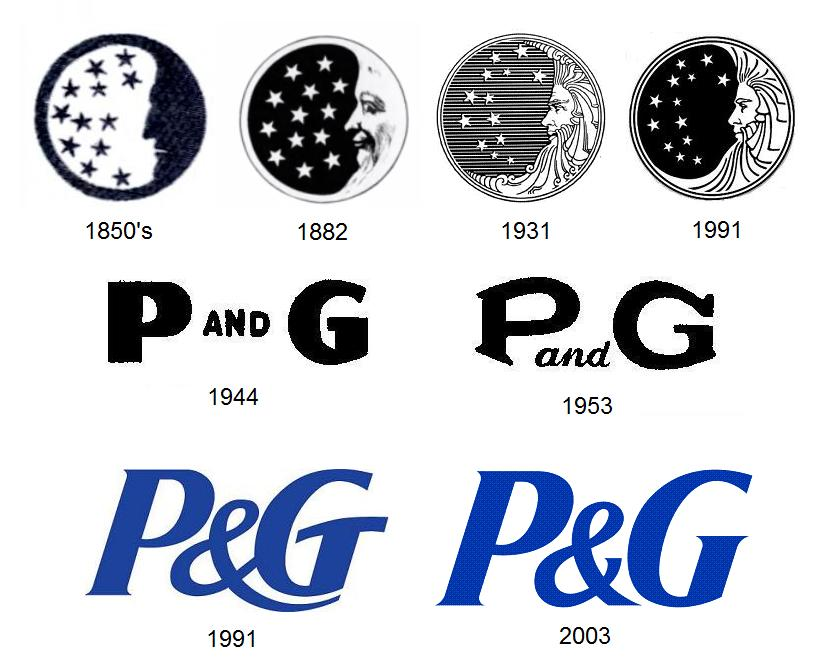
\includegraphics[width=.5\linewidth]{images/supplement/emblemetrics/pg2003}
  \caption{Логотипы P\&G до 2003}
  \label{fig:emblemetrics:pg2003}
\end{figure}

\begin{figure}[ht]
  \centering
  
\includegraphics[width=.5\linewidth]{images/supplement/emblemetrics/pg2013}
  \caption{Обновлённый логотип P\&G 2013}
  \label{fig:emblemetrics:pg2013}
\end{figure}

\begin{figure}[ht]
  \centering
  
\includegraphics[width=.5\linewidth]{images/supplement/emblemetrics/frankenmarks}
  \caption{Frankenmarks}
  \label{fig:emblemetrics:frankenmarks}
\end{figure}

\begin{figure}[ht]
  \centering
  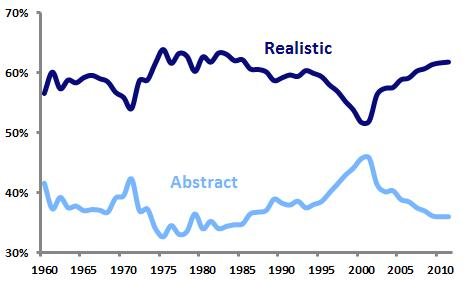
\includegraphics[width=.5\linewidth]{images/supplement/emblemetrics/abstractrealistic}
  \caption{Abstract and realistic logos as a percentage of all new US logos}
  \label{fig:emblemetrics:abstract-realistic}
\end{figure}

\begin{figure}[ht]
  \centering
  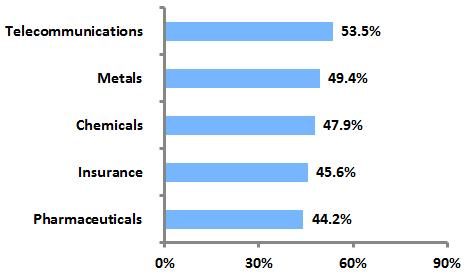
\includegraphics[width=.5\linewidth]{images/supplement/emblemetrics/highabstract}
  \caption{Industries with high rates of abstract logo use}
  \label{fig:emblemetrics:high-abstract}
\end{figure}

\begin{figure}[ht]
  \centering
  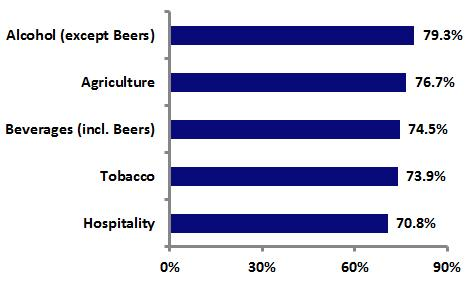
\includegraphics[width=.5\linewidth]{images/supplement/emblemetrics/highrealistic}
  \caption{Industries with high rates of realistic logo use}
  \label{fig:emblemetrics:high-realistic}
\end{figure}

\begin{figure}[ht]
  \centering
  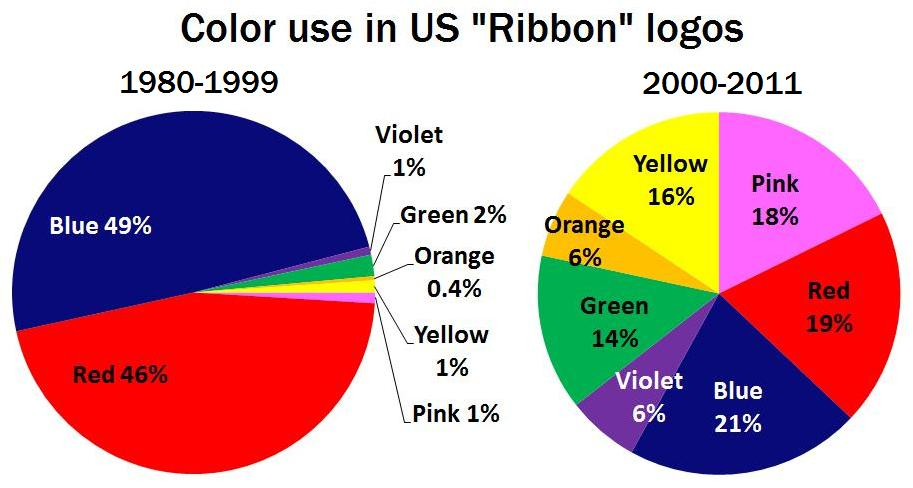
\includegraphics[width=.5\linewidth]{images/supplement/emblemetrics/coloruse}
  \caption{Color use in US Ribbon logos}
  \label{fig:emblemetrics:color-use}
\end{figure}

\begin{figure}[ht]
  \centering
  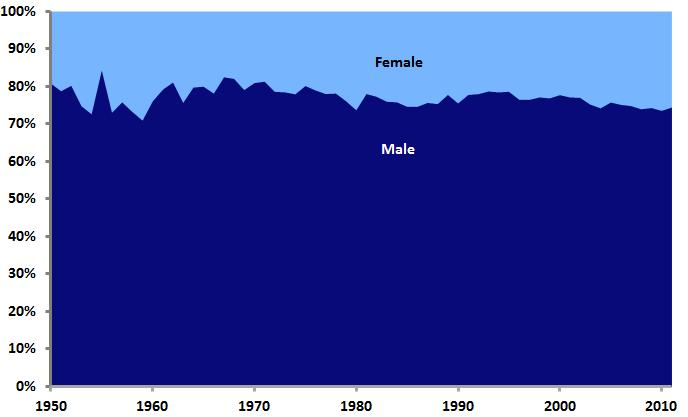
\includegraphics[width=.5\linewidth]{images/supplement/emblemetrics/malefemale}
  \caption{Percentage of new <<gendered>> logos featuring male or female design elements}
  \label{fig:emblemetrics:male-female}
\end{figure}

\begin{figure}[ht]
  \centering
  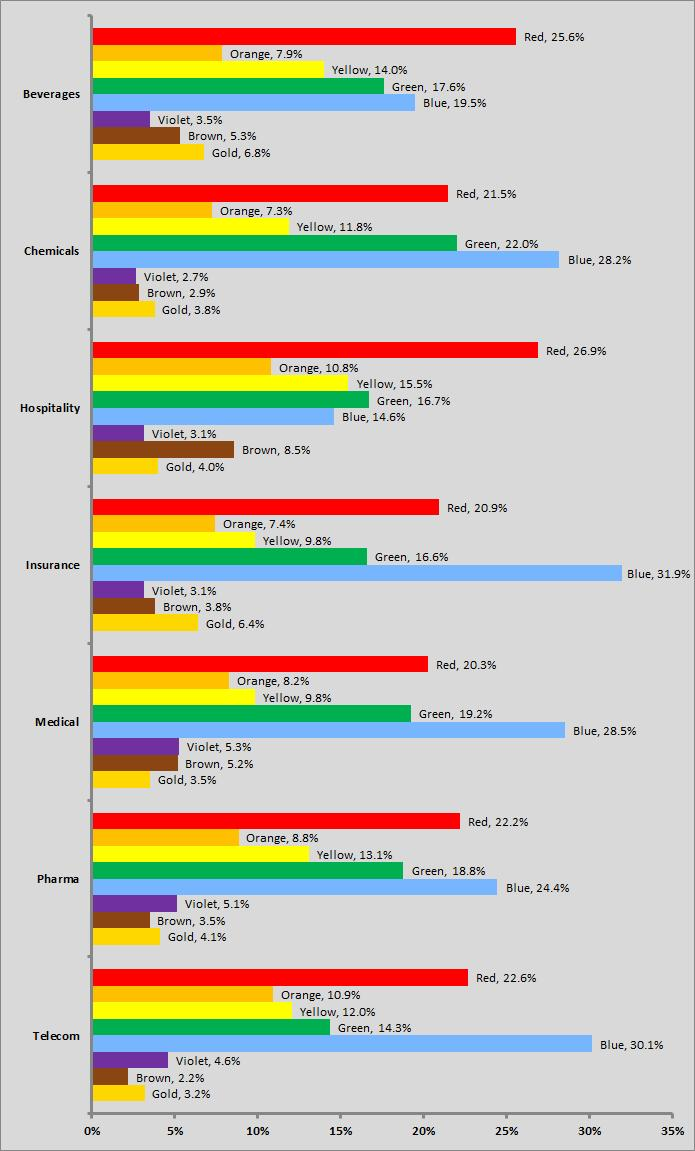
\includegraphics[width=.5\linewidth]{images/supplement/emblemetrics/colorindustry}
  \caption{Use of Color in US Logos by Industry}
  \label{fig:emblemetrics:color-industry}
\end{figure}

\begin{figure}[ht]
  \centering
  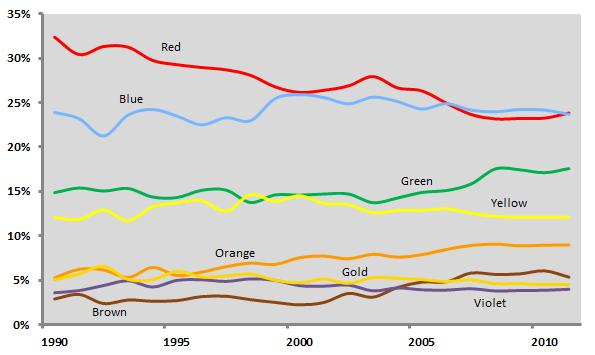
\includegraphics[width=.5\linewidth]{images/supplement/emblemetrics/color}
  \caption{Use of Color in US Logos}
  \label{fig:emblemetrics:color}
\end{figure}

\begin{figure}[ht]
  \centering
  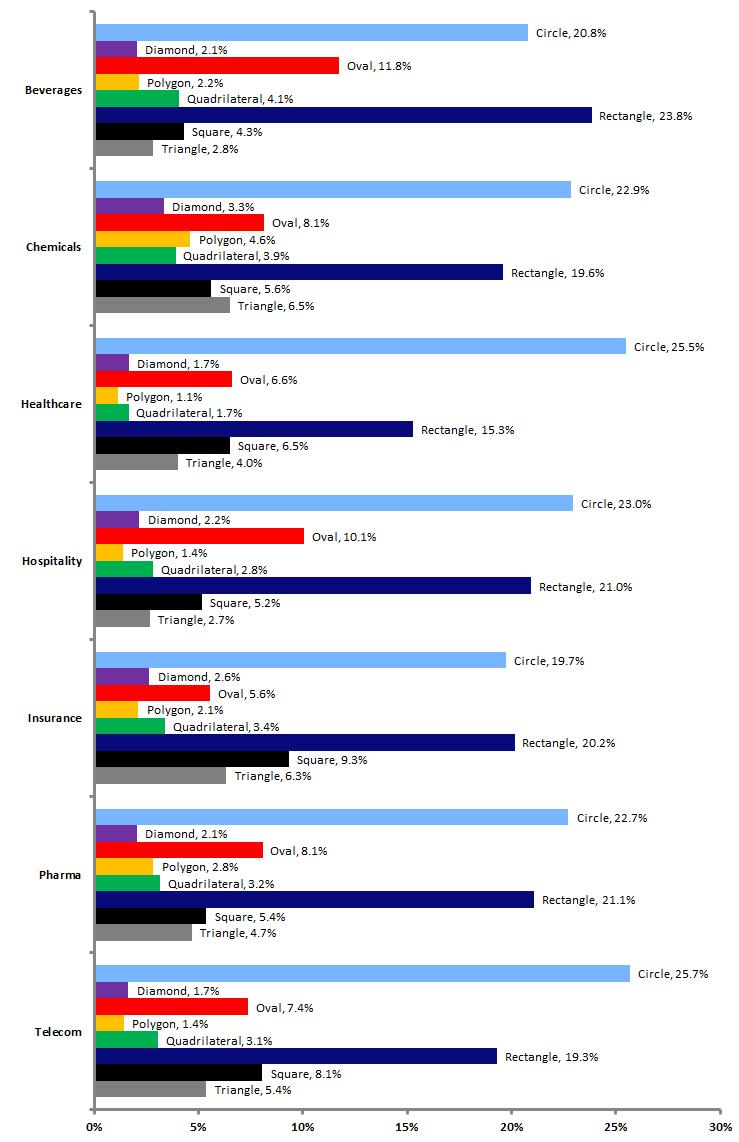
\includegraphics[width=.5\linewidth]{images/supplement/emblemetrics/shapeindustry}
  \caption{Percentage of logos featuring shape elements by industry}
  \label{fig:emblemetrics:shape-industry}
\end{figure}

\begin{figure}[ht]
  \centering
  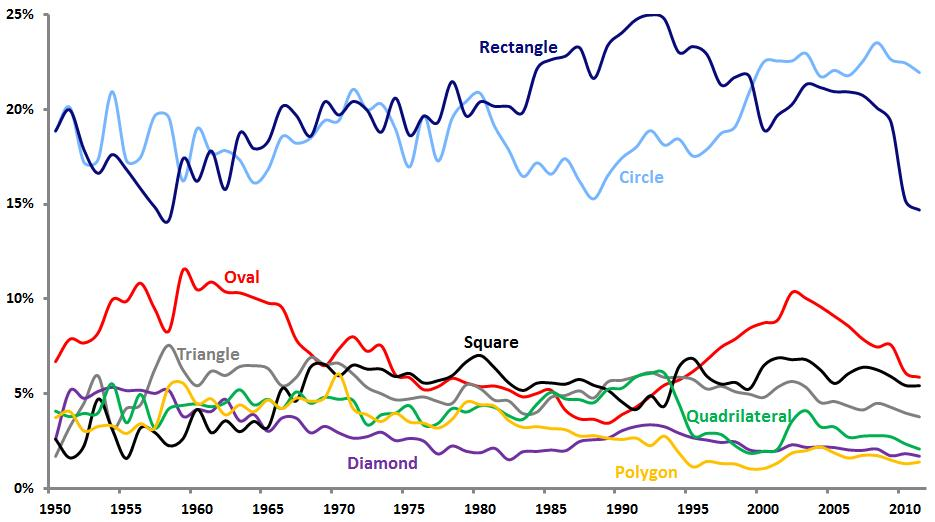
\includegraphics[width=.5\linewidth]{images/supplement/emblemetrics/shape}
  \caption{Percentage of new logos featuring specific shape elements}
  \label{fig:emblemetrics:shape}
\end{figure}

\begin{figure}[ht]
  \centering
  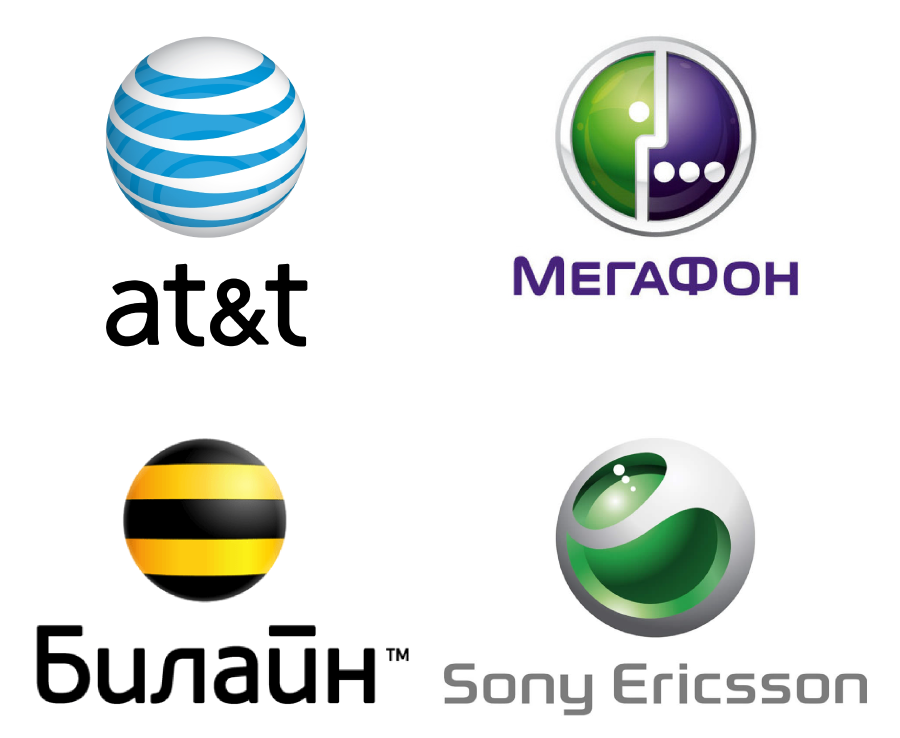
\includegraphics[width=.5\linewidth]{images/supplement/emblemetrics/web20}
  \caption{Логотипы операторов сотовой связи, выполненные в стилистике веб 2.0}
  \label{fig:emblemetrics:web20}
\end{figure}

  \section{Территориальный брендинг}
\label{app:territorial}

\begin{figure}[ht]
  \centering
  
\includegraphics[width=.3\linewidth]{images/supplement/territorial/ny}
  \caption{Логотип-слоган <<I love New York>>, Милтон Глейзер, 1977 г.}
  \label{fig:territorial:ny}
\end{figure}

\begin{figure}[ht]
  \centering
  
\includegraphics[width=.5\linewidth]{images/supplement/territorial/moscow}
  \caption{Логотип сети книжных магазинов <<Москва>>}
  \label{fig:territorial:moscow}
\end{figure}

\begin{figure}[ht]
  \centering
  
\includegraphics[width=.5\linewidth]{images/supplement/territorial/melbourne}
  \caption{Ребрендинг Мельбурна (Австралия), дизайн Джейсон Литтл, Landor Австралия}
  \label{fig:territorial:melbourne}
\end{figure}

\begin{figure}[ht]
  \centering
  
\includegraphics[width=.5\linewidth]{images/supplement/territorial/amsterdam}
  \caption{Амстердам}
  \label{fig:territorial:amsterdam}
\end{figure}

\begin{figure}[ht]
  \centering
  
\includegraphics[width=.5\linewidth]{images/supplement/territorial/copenhagen}
  \caption{Копенгаген}
  \label{fig:territorial:copenhagen}
\end{figure}

\begin{figure}[ht]
  \centering
  
\includegraphics[width=.3\linewidth]{images/supplement/territorial/perm}
  \caption{Логотип г. Пермь, Артемий Лебедев, 2009 г.}
  \label{fig:territorial:perm}
\end{figure}

\begin{figure}[ht]
  \centering
  
\includegraphics[width=.5\linewidth]{images/supplement/territorial/yaroslavl}
  \caption{Логотип г. Ярославль}
  \label{fig:territorial:yaroslavl}
\end{figure}

\begin{figure}[ht]
  \centering
  
\includegraphics[width=.5\linewidth]{images/supplement/territorial/kaluga}
  \caption{Логотип Калужскаой области}
  \label{fig:territorial:kaluga}
\end{figure}

\begin{figure}[ht]
  \centering
  
\includegraphics[width=.3\linewidth]{images/supplement/territorial/nevinnomisk}
  \caption{Логотип г. Невинномысск}
  \label{fig:territorial:nevinnomisk}
\end{figure}

\begin{figure}[ht]
  \centering
  
\includegraphics[width=.2\linewidth]{images/supplement/territorial/omsk}
  \caption{Альтернативный логотип г. Омск}
  \label{fig:territorial:omsk}
\end{figure}

\end{appendices}
\end{document}
